\section{项目功能扩充}
\begin{frame}
    \frametitle{增加单词的数量}
    \footnotesize
    {编译器支持的所有关键字在TokenType.inc中定义,可进入源码查看}
\end{frame}

\begin{frame}
    \frametitle{将整常数扩充为实常数}
    \footnotesize
    {本次项目开发中实现的词法分析器已经能够支持按照C语言语法标准读入实常数,包括整形数和浮点数。此处给出所有接受的浮点表示形式如下:}
    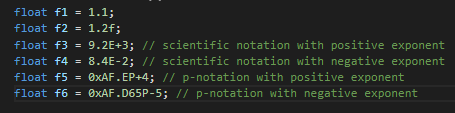
\includegraphics[width=\textwidth]{contents/figure/float.png}
\end{frame}

\begin{frame}
    \frametitle{增强编译器的编译能力}
    \footnotesize
    {编译器在基础项目开发要求的基础上扩展了编译能力,支持包括数组、指针、GCC风格内联汇编语句等等一系列基本C语言语法规范,具体支持的所有C语言语句可以到源码下的test.c测试源码文件中查看}
\end{frame}

\begin{frame}
    \frametitle{较为完善的错误处理}
    \footnotesize
    {对于输入的源码文件,编译器能够给出存在词法错误的token(包括错误类型和位置)还有存在语法错误的语句(包括错误类型和位置),便于开发人员定位错误并且修改}
\end{frame}

\begin{frame}
    \frametitle{从词法分析到可执行文件生成的全套解决方案}
    \footnotesize
    {本编译器最终生成的目标代码文件(例如x86-64汇编或者x86汇编),可以直接输入到对应的第三方编译环境中(例如GCC,Clang等),进一步通过第三方编译环境提供的链接器与第三方实现的标准类库进行链接,最终生成能够在对应平台上正确执行的可执行文件,从而更加直观地查看编译器对于源码逻辑编译的正确性}
\end{frame}